\documentclass{article}
\usepackage{graphicx}
\usepackage{tcolorbox}
\usepackage{url}
\usepackage{bdd}
\usepackage[utf8]{inputenc}

\newcommand{\instruction}[1]{\textsc{\begin{tcolorbox}#1\end{tcolorbox}}}

\begin{document}

\title{[Título del Proyecto] (Numero del Grupo)}
\author{[Nombres de Estudiantes]}

\maketitle

% descommentar la siguiente línea para borrar los cuadros
% \renewcommand{\instruction}[1]{}
\instruction{Se pueden borrar los cuadros grises del informe final.}

\section{Datos}

\instruction{Describan el tema, el fuente (URL), el formato (CSV, JSON, etc.), el alcance y algunas estadísticas interesantes (tamaño, numero de lineas, etc.) de los datos crudos. Si uds.\ tuvieron que hacer algún tipo de pre-procesamiento (parsear datos, extraer datos, etc.), también se puede describir este proceso aquí. [aprox.\ $\frac{1}{2}$ página]:}

\medskip
El tema de los datos es ...

\section{Esquema Relacional}

\instruction{Presenten el esquema relacional, incluyendo el esquema de las tablas usadas, las llaves primarias/foráneas, restricciones, etc. (No hay que dar el SQL para crear las tablas, solo hay que describir el esquema.) [aprox. $\frac{1}{2}$ page]:}

\medskip
En la figura~\ref{fig:esquema}, se representa el esquema relacional que contiene tres tablas ...

\begin{figure}[h]
\begin{center}
	\sf
	\footnotesize
	\rlt{Cervezas}(\schk{nombre}\dstr,\sch{tipo}\dstr,\sch{grados}\dfl,\sch{ciudad-origen}\dstr)\\
	\rlt{Vinos}(\schk{nombre}\dstr,\sch{tipo}\dstr,\sch{año}\dint,\sch{grados}\dfl,\sch{ciudad-origen}\dstr)\\
	\rlt{En-Stock}(\schk{nombre}\dstr,\schk{fecha}\dom{date},\sch{cantidad}\dint,\sch{precio-unitario}\dint)\\
	
% usa \dom{date} para otros tipos
\end{center}

\caption{El esquema relacional del proyecto (ejemplo)}\label{fig:esquema}
\end{figure}

\section{Indíces, Vistas, etc.}

\instruction{Describen los indices, las vistas, los gatillos, u otras características de SQL usadas en el proyecto. (No hay que dar los comandos de SQL; solo hay que describir las características y motivar su uso.) [aprox.\ $\frac{1}{2}$ página]:}

\medskip
Usamos un indice del tipo X sobre tabla Y porque ...

\section{Consultas}

\instruction{Describen las consultas bases usadas en el proyecto para crear la aplicación. Hay que dar las consultas en SQL, motivarlas un poco (¿por qué son interesantes?) y describir su función [aprox. $\frac{1}{2}$ página de discusión sin considerar el espacio tomado por las consultas en SQL].}

En total tenemos X consultas:

\begin{enumerate}
	\item La primera consulta está en la figura~\ref{fig:c1}. Usamos esta consulta para ...
	\item ...
	\item ...
\end{enumerate}

\begin{figure}[h]
	\lstset{language=SQL,style=sqlq}
	\begin{lstlisting}
	SELECT s1.nombre AS nombre1,
	s2.nombre AS nombre2
	FROM Satélite s1,Satélite s2
	WHERE s1.año=?
	AND s1.nombre<?
	\end{lstlisting}
	
	\caption{Consulta 1 (ejemplo)}\label{fig:c1}
\end{figure}

\section{Implementación de la Aplicación}

\instruction{Describen el proceso de implementar la aplicación: que software usaron, cómo implementaron la conexión a la base de datos, cómo implementaron la aplicación Web, cómo  aseguraron la seguridad del sistema contra inyecciones, etc. Con respecto a la seguridad, hay que dar un fragmento de código donde se crea(n) y se manda(n) la(s) consultas a la base de datos. [aprox.\ $\frac{1}{2}$ página de discusión].}

Usamos X libraría para conectar a la base de datos. Se implementa la aplicación en lenguaje Y con Z como servidor Web. En la figura~\ref{fig:codigo}, se lista el código para crear y mandar una consulta a la base de datos. ...

\begin{figure}[h]
	\begin{verbatim}
	public static int consultar(String stringEntrada) {
	   Statement stmt = ...
	}
	\end{verbatim}
	\caption{El código para consultar la base de datos (ejemplo)}
	\label{fig:codigo}
\end{figure}

\section{Ejemplos de la Aplicación}

\instruction{Den algunos ejemplos concretos de búsqueda usando su aplicación con los resultados. Se pueden incluir \textit{screenshots}. Hay que incluir un enlace a la aplicación tambíen. [aprox.\ $\frac{1}{2}$ página de discusión sin considerar el espacio tomado por los screenshots].}

La aplicación está disponible aquí: \url{http//miapp.com/example/}.

El usuario puede hacer consultas como ... 

En la figura~\ref{fig:s1}, se muestra la interfaz para hacer consultas donde ...

En la figura XX, se muestra ejemplos de resultados para una búsqueda ...

\begin{figure}[h]
	\centering
	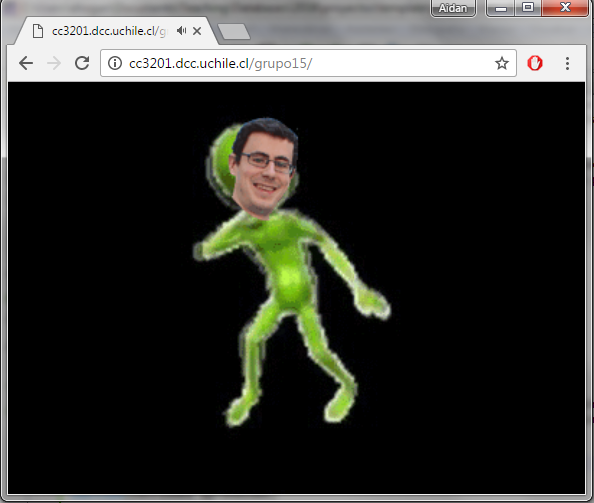
\includegraphics[scale = 0.6]{screenshot}
	\caption{El \textit{screenshot} de la página inicial (ejemplo)}
	\label{fig:s1}
\end{figure}

\section{Lecciones aprendidas}

\instruction{¿Qué fue difícil? ¿Qué fue fácil? ¿Algo interesante? ¿Qué aprendieron? [aprox. $\frac{1}{2}$ página]}





\end{document}